\subsection{Đề 2}
\Opensolutionfile{ans}[ans/ans-2-B5.2]
\caulc
\begin{ex}%[2D1V3-6]
Một vật chuyển động theo quy luật $s=-\dfrac{1}{3}t^3+6t^2$ với $t$ (giây) là khoảng thời gian tính từ khi vật bắt đầu chuyển động và $s$ (mét) là quãng đường vật di chuyển được trong khoảng thời gian đó. Hỏi trong khoảng thời gian $7$ giây, kể từ khi bắt đầu chuyển động, tốc độ lớn nhất của vật đạt được bằng bao nhiêu?
\choice
{$24$ m/s}
{\True $36$ m/s}
{$180$ m/s}
{$144$ m/s}
\loigiai{
Công thức vận tốc chuyển động của vật là $ v(t)=s'(t)=-t^2+12t$.\\
Trên khoảng $[0;7]$ ta có $v(t) =36-(t^2-12t+36) =36-\left( t-6 \right)^2 \leq 36$ (m/s).\\
Do đó $\max\limits_{[0;7]} v(t)=36 \Leftrightarrow t=6$.\\
Vậy tốc độ lớn nhất của vật trong khoảng thời gian $7$ giây, kể từ khi bắt đầu chuyển động là $36$ m/s.
}
\end{ex}

\begin{ex}%[2D1V3-6]
 Một đoàn tàu chuyển động thẳng khởi hành từ một nhà ga. Quãng đường (theo đơn vị mét (m)) đi được của đoàn tàu là một hàm số của thời gian $t$ (theo đơn vị giây (s)) cho bởi phương trình là $S=6t^2-t^3$. Tìm thời điểm $t$ mà tại đó tốc độ $v$(m/s) của đoàn tàu là lớn nhất?
\choice
{$t=4$ s}
{$t=1$ s}
{\True $t=2$ s}
{$t=6$ s}
\loigiai{
 Ta có $v(t)=s'(t)=12t-3t^2=12-3(t-2)^2\leq 12$.\\
 Vậy $v(t)$ đạt giá trị lớn nhất tại $t=2$ giây.
}
\end{ex}

\begin{ex}%[2D1V3-6]
Sau khi phát hiện một bệnh dịch, các chuyên gia y tế ước tính số người nhiễm bệnh kể từ ngày xuất hiện bệnh nhân đầu tiên đến ngày thứ $t$ là  $f(t) =15t^2 -t^3$ (theo kết quả khảo sát các năm vừa qua). Nếu xem $f'(t)$ là tốc độ truyền bệnh (người/ngày) tại thời điểm $t$ thì vào ngày mà tốc độ truyền bệnh lớn nhất, số người nhiễm bệnh là bao nhiêu?
\choice
{$500$}
{\True $250$}
{$600$}
{$75$}
\loigiai{
Ta có $f'(t) = -3t^2 +30t$ và $f''(t) = -6t + 30$.\\
Lại có $f''(t) =0 \Leftrightarrow t=5$.\\
Bảng biến thiên của hàm số $f'(t)$ ($t>0$).
\begin{center}

\begin{tikzpicture}
\tkzTabInit[lgt=1.2,espcl=2.5]
  {$t$  /1.0, $f''(t)$ /1.0,$f'(t)$ /2.2}
  {$0$ , $5$ ,$+\infty$}
\tkzTabLine{,+,0,-,}
\tkzTabVar{-/$0$ ,+/$75$, -/$-\infty$}
\end{tikzpicture}
\end{center}
Vậy vào ngày tốc độ truyền bệnh lớn nhất, số người nhiễm bệnh là $f(5)=250$ người.
}
\end{ex}

\begin{ex}%[2D1V3-6]
Một công ty bất động sản có $40$ căn hộ cho thuê. Biết rằng nếu cho thuê mỗi căn hộ với giá $3\,000\,00$ đồng một tháng thì mọi căn hộ đều có người thuê và cứ tăng thêm giá mỗi căn hộ $100\,000$ đồng một tháng (theo quy định trong hợp đồng) thì sẽ có một căn hộ bị bỏ trống. Hỏi muốn có thu nhập cao nhất thì công ty đó phải cho thuê mỗi căn hộ với giá bao nhiêu một tháng?
\choice
{\True $3\,500\,000$ đồng}
{$4\,000\,000$ đồng}
{$3\,700.000$ đồng}
{$3\,900\,000$ đồng}
\loigiai{
Gọi $x$ là số căn hộ bị bỏ trống $\left(0 \le x \le 40\right)$.\\
Vậy giá cho thuê một căn phòng là $3+0{,}1x$ (triệu đồng).\\
Số căn hộ cho thuê là $40-x$. \\
Số tiền thu được là 
$$T=(40-x) \cdot (3+0{,}1x)=-0{,}1x^2+x+120 \Rightarrow T'=-0{,}2x+1 \Rightarrow T'=0 \Rightarrow x=5.$$
Ta có bảng biến thiên
\begin{center}

\begin{tikzpicture}
\tkzTabInit[espcl=2.5,lgt=1.5]
{$x$/0.7,$T'$/0.7,$T$/2.1}
{$0$,$5$,$40$}
\tkzTabLine{,+,0,-,}
\tkzTabVar{-/$ $,+/$ 3\,500\,000 $,-/$ $}
\end{tikzpicture}
\end{center}
Vậy $T$ đạt giá trị lớn nhất khi $x=5$, khi đó giá thuê một căn phòng là $3\,500\,000$ đồng.
}
\end{ex}

\begin{ex}%[2D1V3-6]
Một chất điểm chuyển động có vận tốc tức thời $v(t)$ phụ thuộc vào thời gian $t$ theo hàm số $v(t)=-t^4+24t^2+500$ (m/s). Trong khoảng thời gian từ $t=0$ (s) đến $t=10$ (s) chất điểm đạt tốc độ lớn nhất tại thời điểm nào (làm tròn kết quả đến hàng đơn vị)?
\choice
{$t=2$}
{\True $t=4$}
{$t=0$}
{$t=1$}
\loigiai{
Ta có $v'(t)=-4t^3+48t=-4t(t^2-12)$.\\
Xét phương trình $v'(t)=0\Leftrightarrow \hoac{&t=0\\&t=\pm 2\sqrt{3}.}$\\
Bài toán trở thành tìm giá trị lớn nhất của hàm số $v(t)$ trên đoạn $[0;10]$, ta có
$$v(0)=500, v(2\sqrt{3})=664, v(10)=-9260.$$
Vậy tốc độ lớn nhất khi $t=2\sqrt{3}\approx 4$ (s).
}
\end{ex}

\begin{ex}%[2D1V3-6]
\immini{
Từ một tấm tôn có hình dạng là nửa hình tròn bán kính $R=3$, người ta muốn cắt ra một hình chữ nhật (hình vẽ bên). Diện tích lớn nhất có thể của tấm tôn hình chữ nhật là
\choice
{$\dfrac{9}{2}$}
{$6\sqrt2$}
{$9\sqrt2$}
{\True $9$}
}
{
\begin{tikzpicture}[thick,scale=0.7]
\draw [-] (-4,0)--(4,0);
\draw [-] (-3,0)--(-2.99,2.65)--(2.99,2.65)--(3,0);
\draw[smooth,samples=200,variable=\t,domain=0:180] plot({(4)*cos (\t)},{(4)*sin(\t)});
\draw (0,0) [fill=black] circle (1pt) node[below]{$O$};
\draw (-3,0) [fill=black] circle (1pt) node[below]{$Q$};
\draw (3,0) [fill=black] circle (1pt) node[below]{$P$};
\draw (-2.99,2.65) [fill=black] circle (1pt) node[left]{$M$};
\draw (2.99,2.65) [fill=black] circle (1pt) node[right]{$N$};
\draw[pattern=north east lines,pattern color=black!50!] (-3,0)--(-2.99,2.65)--(2.99,2.65)--(3,0);
\end{tikzpicture}
}
\loigiai{
Đặt $OQ=x,\ (0<x<3) \Rightarrow MQ=\sqrt{MO^2-OQ^2}=\sqrt{9-x^2}$.\\
Ta có  $S_{MNPQ}=PQ\cdot MQ=2x\cdot\sqrt{9-x^2}\le 2\cdot\dfrac{x^2+9-x^2}{2}=9.$\\
Dấu $''=''$ xảy ra khi $x=\dfrac{3\sqrt2}{2}.$\\
Vậy diện tích lớn nhất của tấm tôn bằng $9$.
}
\end{ex}

\begin{ex}%[2D1V3-6]
Một xưởng sản xuất những thùng hình hộp chữ nhật bằng nhôm không nắp và có các kích thước $x, y, z$ (dm). Biết tỉ số hai cạnh đáy là $x:y=1:3$, thể tích khối hộp bằng $18\,\text{dm}^3$. Để tốn ít vật liệu nhất thì tổng $x+y+z$ bằng
\choice
{$10$ dm}
{$\dfrac{26}{3}$ dm}
{$26$ dm}
{\True $\dfrac{19}{2}$ dm}
\loigiai{
Thể tích khối hộp là $V=xyz=3x^2z=18\Rightarrow z=\dfrac{6}{x^2}$.\hfill $(1)$\\
Diện tích nhôm cần sử dụng để sản xuất khối hộp là $S=xy+2(yz+zx)$.\hfill $(2)$\\
Thay $(1)$ vào $(2)$ ta có $S=3x^2+\dfrac{48}{x}$ suy ra $S'=6x-\dfrac{48}{x^2}$.\\
Xét phương trình $S(x)=0\Leftrightarrow 6x-\dfrac{48}{x^2} = 0\Leftrightarrow  x=2$.\\
Vẽ bảng biến thiên ta thấy $S$ đạt giá trị nhỏ nhất khi $x=2$, $y=6$, $z=\dfrac{3}{2}$.\\
Khi đó $x+y+z=\dfrac{19}{2}$.
}
\end{ex}

\begin{ex}%[2D1V3-6]
Ông An muốn xây một bể nước dạng hình hộp chữ nhật có nắp với dung tích $3000$  lít. Đáy bể là một hình chữ nhật có chiều dài gấp đôi chiều rộng. Giá thuê nhân công để xây hồ là  $500\,000$ đồng cho mỗi mét vuông. Hỏi chi phí thấp nhất ông An cần bỏ ra để xây bể nước là bao nhiêu?
\choice
{\True  $6\,490\,123$ đồng}
{$5\,151\,214$ đồng}
{ $7\,500\,000$ đồng}
{$6\,500\,000$ đồng}
\loigiai{
Gọi $x$  là chiều rộng bể, chiều dài bể là  $2x$,   diện tích đáy là $2x^2$.\\
Do thể tích bể là $V=3\,000$ lít $=3$ m$^3$  nên chiều cao bể là $\dfrac{3}{2x^2}$ .\\
Diện tích xây dựng là diện tích toàn phần của bể là
$$ S=2\left(2x^2+x\cdot \frac{3}{2x^2}+2x\cdot \frac{3}{2x^2}\right)=2\left(2x^2+\frac{9}{2x}\right)=4x^2+\frac{9}{2x}+\frac{9}{2x}\geq 3\sqrt[3]{81}.$$
Vậy diện tích xây dựng ít nhất là $S=9\sqrt[3]{3}$  khi và chỉ khi $4x^2=\dfrac{9}{2x}\Leftrightarrow x=\dfrac{\sqrt[3]{9}}{2}$.\\
Chi phí xây dựng ít nhất là $9\sqrt[3]{3} \cdot 500000 \approx 6\,490\,123$  đồng.
}
\end{ex}

\begin{ex}%[2D1V3-6]
Một thanh sắt chiều dài $AB=100$ m được cắt thành hai phần $AC$ và $CB$ với $AC=x$ (m). Đoạn $AC$ được uốn thành một hình vuông có chu vi bằng $AC$ và đoạn $CB$ uốn thành tam giác đều có chu vi bằng $CB$. Khi tổng diện tích của hình vuông và tam giác nhỏ nhất, mệnh đề nào dưới đây đúng?
\begin{center}
\begin{tikzpicture}[scale=0.7, font=\footnotesize,line join=round, line cap=round,>=stealth]
\draw (-6,0)circle (1pt) node[left]{$A$}--(1,0)circle (1pt) node[above]{$C$}--(6,0)circle (1pt) node[right]{$B$};
\draw[->] (0,-0.3)--(-2,-1.8);
\draw[->] (0,-0.3)--(2,-1.8);
\draw (-3,-2)--(-1,-2)--(-1,-4)--(-3,-4)--cycle;
\draw (2,-2)--(0.7,-4)--(3.3,-4)--cycle;
\end{tikzpicture}
\end{center}
\choice
{$x\in (52;58)$}
{$x\in (48;52)$}
{\True $x\in (40;48)$}
{$x\in (30;40)$}
\loigiai{
Theo đề các cạnh của hình vuông có độ dài là $\dfrac{x}{4}$, các cạnh của tam giác đều có độ dài là $\dfrac{100-x}{3}$.\\
Ta có $S=\left(\dfrac{x}{4} \right)^2+\left(\dfrac{100-x}{3}\right)^2\cdot\dfrac{\sqrt{3}}{4}= \dfrac{\left( 9+4\sqrt{3}\right)}{144} x^2-\dfrac{800\sqrt{3}}{144}x+\dfrac{40000\sqrt{3}}{144}.$\\
Đây là hàm bậc hai có hệ số $a>0$ nên hàm đạt giá trị nhỏ nhất khi $$x=-\dfrac{b}{2a}=\dfrac{800\sqrt{3}}{144}\cdot \dfrac{144}{2\cdot(9+4\sqrt{3})}\approx 43{,}5 \text{ m}.$$
}
\end{ex}

\begin{ex}%[2D1V3-6]
Một người bán buôn Thanh Long Đỏ nhận thấy rằng: Nếu bán với giá $20\,000$ đồng/kg thì mỗi tuần có $90$ khách đến mua và mỗi khách mua trung bình $60$ kg. Cứ tăng giá $2\,000$ đồng/kg thì số khách mua hàng tuần giảm đi $1$ và khi đó mỗi khách lại mua ít hơn mức trung bình $5$ kg, và như vậy cứ giảm giá $2\,000$ đồng/kg thì số khách mua hàng tuần tăng thêm $1$ và khi đó mỗi khách lại mua nhiều hơn mức trung bình $5$ kg. Hỏi người đó phải bán với giá mỗi kg là bao nhiêu để lợi nhuận thu được hàng tuần là lớn nhất, biết rằng người đó phải nộp tổng các loại thuế là $2\,200$ đồng/kg (kết quả làm tròn đến hàng nghìn).
\choice
{$16\,000$ đ}
{$12\,000$ đ}
{$24\,000$ đ}
{\True $22\,000$ đ}
\loigiai{
Giả sử giá bán thay đổi $x$ lần, mỗi lần thay đổi $2\,000$ đồng ($x\in\mathbb{Z}$, $x>0$ là tăng giá, $x<0$ là giảm giá).\\
Theo thực tế thì $-10<x<45$ (giá bán trên $0$ đồng và còn ít nhất một khách).\\
Tổng tiền thu được sau khi thay đổi là \\
$T=(90-x)(60-5x)(20+2x-2{,}2)=10x^3-931x^2+1772x+96120$.\\
Xét hàm số $T(x)=10x^3-931x^2+1772x+96120$.\\
Bài toán trở thành tìm GTLN của $T(x)$ với $x\geq 20\,000$.\\
Ta có $T'(x)=30(x^2-62\text{,}0667x+57\text{,}4)$.\\
$T'=0\Leftrightarrow \hoac{&x\approx 1\\&x\approx 61.}$\\
Bảng biến thiên của $T(x)$
\begin{center}
\begin{tikzpicture}
\tkzTabInit[lgt=1.2,espcl=3]
{$x$  /1.2, $T'(x)$ /1.2,$T(x)$  /2.0}
{$-10$ , $1$, $45$}
\tkzTabLine{,+,z,-,}
\tkzTabVar{-/,+/$T_\text{CĐ}$, -/}
\end{tikzpicture}
\end{center}
Dựa vào bảng biến thiên suy ra $T$ lớn nhất khi $x=1$, tức là ta chỉ tăng giá một lần.\\
Vậy giá bán đưa ra để lợi nhuận cao nhất là $22\,000$.
}
\end{ex}

\begin{ex}%[2D1C3-6]
Trên sa mạc có một khu đất hình chữ nhật $ABCD$ có chiều dài $AB=70$ km, chiều rộng $AD=10$ km. Vận tốc trung bình của xe máy trên khu đất này là $20$ km/h, riêng đi trên cạnh $CD$ thì vận tốc là $40$ km/h. Một người đi xe máy xuất phát từ $A$ muốn đến $B$ thì cần ít nhất bao nhiêu giờ?
\choice
{$\dfrac{7}{2}$}
{\True $\dfrac{2\sqrt{3}+7}{4}$}
{$\dfrac{10}{\sqrt{3}}$}
{$\dfrac{20}{\sqrt{3}}$}
\loigiai{
\immini{
$\bullet$ Nếu không đi trên cạnh $CD$ thì cách di chuyển nhanh từ $A$ đến $B$ là di chuyển trên đoạn $AB$, khi đó mất $3{,}5$ giờ.\\
$\bullet$ Nếu có di chuyển trên $CD$ giả sử từ $A$ đi đến $M$, $M$ đến $N$ và $N$ đến $B$ (như hình vẽ).\\
Đặt $MD=m$, $NC=n$. Ta có thời gian di chuyển từ $A$ đến $B$ là
$$t=\dfrac{\sqrt{100+m^2}+\sqrt{100+n^2}}{20}+\dfrac{70-(m+n)}{40}.$$
}{
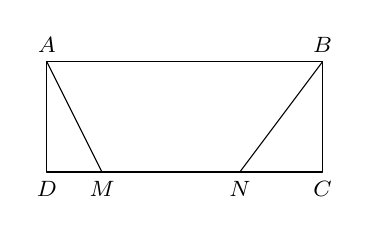
\begin{tikzpicture}[scale=0.7, font=\footnotesize,line join=round, line cap=round,>=stealth]
\draw (0,0) rectangle (5,-2);
\path
(0,0) node[above]{$A$} (5,0) node[above]{$B$}
(5,-2) node[below]{$C$} (3.5,-2) node[below]{$N$} (1,-2) node[below]{$M$} (0,-2) node[below]{$D$};
\draw (0,0) -- (1,-2);
\draw (5,0) -- (3.5,-2);
\end{tikzpicture}
}
\noindent Áp dụng bất đẳng thức $\sqrt{a^2+b^2}+\sqrt{c^2+d^2} \ge \sqrt{(a+c)^2+(b+d)^2}$, ta có
$$t \ge \dfrac{\sqrt{20^2+(m+n)^2}}{20}+\dfrac{70-(m+n)}{40},$$
dấu \lq \lq $=$\rq \rq \, xảy ra khi và chỉ khi $m=n$.\\
Đặt $m+n=x$, xét hàm $f(x)=\dfrac{\sqrt{400+x^2}}{20}+\dfrac{70-x}{40},~x \in (0,70]$.\\
Ta có $f'(x)=\dfrac{x}{20\sqrt{400+x^2}}-\dfrac{1}{40},~x \in [0,70]$.
\[ f'(x)=0 \Leftrightarrow \sqrt{400+x^2}=2x \Leftrightarrow x=\dfrac{20}{\sqrt{3}}.\]
Bảng biến thiên của $f(x)$
\begin{center}

\begin{tikzpicture}[scale=1, font=\footnotesize,line join=round, line cap=round,>=stealth]
\tkzTabInit[nocadre=false,lgt=1.2,espcl=2.5,deltacl=0.6]
{$x$/1,$f'(x)$/0.6,$f(x)$/2}
{$0$,$\dfrac{20}{\sqrt{3}}$,$70$}
\tkzTabLine{ ,-,0,+, }
\tkzTabVar{+/$\dfrac{11}{4}$,-/$\dfrac{2\sqrt{3}+7}{4}$,+/$\dfrac{\sqrt{50}}{2}$}
\end{tikzpicture}
\end{center}
$\Rightarrow$ giá trị nhỏ nhất của $f(x)$ là $f\left(\dfrac{20}{\sqrt{3}}\right)=\dfrac{2\sqrt{3}+7}{4}$.\\
Vậy thời gian ngắn nhất là $\dfrac{2\sqrt{3}+7}{4}$ khi $m=n=\dfrac{x}{2}=\dfrac{10}{\sqrt{3}}$.
}
\end{ex}

\begin{ex}%[2D1V3-6]
\immini{
	Máng trượt của một cầu trượt cho trẻ em (\textit{Hình a}) được uốn từ một tấm kim loại có bề rộng $80$ cm, mặt cắt được mô tả ở \textit{Hình b}. Nhà thiết kế khuyến cáo, diện tích mặt cắt càng lớn thì càng đảm bảo an toàn cho trẻ em.
}{
	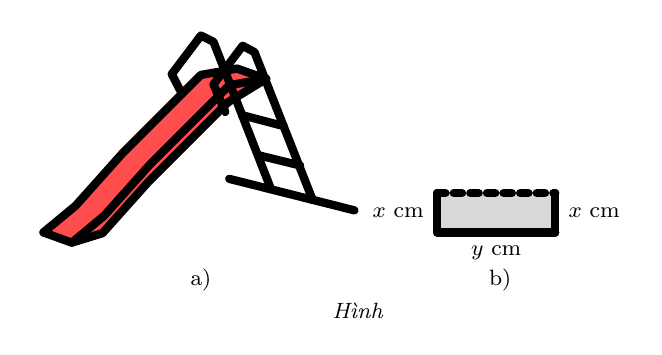
\begin{tikzpicture}[scale=1, font=\footnotesize, line join=round, line cap=round, >=stealth,line width=3.pt]
		\clip(-0.2,-1.2) rectangle (7.5,2.6);
		\fill[line width=3.pt,color=red,fill=red,fill opacity=0.7] (0,0)--(0.41,0.34)--(1,1)--(1.76,1.76)--(2,2)--(2.46,2.08)--(2.83,1.95)--(2.34,1.65)--(1.34,0.65)--(0.75,-0.01)--(0.36,-0.13)-- cycle;
		\draw (0,0)--(0.41,0.34)--(1,1)--(2,2)--(2.46,2.08);
		\draw (0,0)--(0.36,-0.13)--(0.77,0.21)--(0.77,0.21)--(1.36,0.87)--(2.36,1.87)--(2.83,1.95);
		\draw (0.36,-0.13)--(0.75,-0.01)--(1.34,0.65)--(2.34,1.65);
		\draw (2.36,0.68)-- (3.95,0.28);
		\draw (3.42,0.41)--(2.68,2.29)--(2.53,2.37)--(2.16,1.88)--(2.31,1.53);
		\draw (1.63,2.01)--(2,2.5)-- (2.16,2.42)--(2.89,0.55);
		\draw (1.63,2.01)--(1.76,1.76) (2.73,0.98)--(3.26,0.85) (2.52,1.49)--(3.05,1.35);
		\draw (2.34,1.65)--(2.83,1.95)--(2.46,2.08);
		\draw (2,-0.6)node{a)};
		\fill[line width=3.pt,fill=gray,fill opacity=0.3] (5,0.5)--(5,0)--(6.5,0)--(6.5,0.5)--cycle;
		\draw (5,0.5)--(5,0) node [left ,sloped,pos=0.5,rotate=90] {$x$ cm};
		\draw (5,0)--(6.5,0) node [below,sloped,pos=0.5] {$y$ cm};
		\draw (6.5,0)--(6.5,0.5) node [right,sloped,pos=0.5,rotate=-90] {$x$ cm};
		\draw[dashed] (5,0.5)--(6.5,0.5);
		\draw (5.8,-0.6)node{b)};
		\draw (4,-1)node{\textit{Hình }};
	\end{tikzpicture}
	}
\noindent
	Với $x$ đạt giá trị bằng bao nhiêu thì cầu trượt đảm bảo an toàn nhất cho trẻ em?
	\choice
{$x = 16$ cm}
{$x=18$ cm}
{$x=22$ cm}
{\True $x=20$ cm}
	\loigiai{
	Do tấm kim loại có bề rộng $80 \mathrm{~cm}$ nên ta có: $2x+y=80 \Leftrightarrow y=80-2x$.\\
		Để có thể thiết kế được máng trượt thì $y>0 \Leftrightarrow 80-2 x>0 \Leftrightarrow x<40$. Suy ra $0<x<40$.\\
		Diện tích của mặt cắt máng trượt là $S=x y=x(80-2x)=-2x^2+80x$.\\		
	Ta có
		\allowdisplaybreaks
		\begin{eqnarray*}
			S(x)&=&-2x^2+80x \text{ với } x\in(0; 40);\\
			S'(x)&=&-4 x+80 \\
			S'(x)&=&0 \Leftrightarrow-4 x+80=0 \Leftrightarrow x=20.
		\end{eqnarray*}
		Bảng biến thiên của hàm số $S(x)$ như sau
		\begin{center}
			
\begin{tikzpicture}[font=\footnotesize,thick,>=stealth]
				\tikzset{double style/.append style={double distance=1.5pt}}
				\tkzTabInit[nocadre=false,lgt=1.2,espcl=2.5,deltacl=0.6,lw=.75pt,color,colorL=green!50,colorV=green!50]
				{$x$ /0.7, $S'(x)$ /0.8, $S(x)$ /2}
				{$0$,$20$,$40$}
				\tkzTabLine{ ,+,,-, }
				\tkzTabVar{-/$0$,+/$800$,-/$0$}
			\end{tikzpicture}
		\end{center}
	Do đó, hàm số $S(x)$ đạt cực đại tại $x=20$ và $S_{\text{CĐ}}=800$.\\
	Vậy để cầu trượt đảm bảo an toàn nhất cho trẻ em thì $x=20$ (cm).
	}
\end{ex}
\Closesolutionfile{ans}
\indapan{6}{ans/ans-2-B5.2}

\cauds

\Opensolutionfile{ans}[ans/ans-2-B5.2-DS]
\begin{ex}%[2D1V4-4]
Một bể bơi chứa $5\,000$ lít nước tinh khiết. Người ta bơm vào bể đó nước muối có nồng đồ $30$ gam muối cho mỗi lít nước với tốc độ $25$ lít/phút.
\choiceTFt
{\True Sau $t$ phút khối lượng muối trong bể là $750t$ (gam)}
{\True Nồng độ muối trong bể sau $t$ phút (tính bằng tỉ số của khối lượng muối trong bể và thể tích nước trong bể, đơn vị: gam/lít) là $f(t)=\dfrac{30t}{200-t}$}
{\True Xem $y=f(t)$ là một hàm số xác định trên nửa khoảng $[0;+\infty)$,  tiệm cận ngang của đồ thị hàm số đó có phương trình là $y = 30$}
{\True Khi $t$ ngày càng lớn thì nồng độ muối trong bể sẽ tiến gần đến mức $30$ (gam/lít)}
\loigiai{
\immini{Sau $t$ phút, khối lượng muối trong bể là 
\[
	25\cdot 30\cdot t=750t \text{ (gam)}
\]
Thể tích của lượng nước trong bể là $5\,000+25t$ (lít).\\
Vậy nồng độ muối sau $t$ phút là 
   \[
   f(t)=\dfrac{750t}{5\,000+25t}=\dfrac{30t}{200+t}\,\text{(gam/lít)}.
   \]
Ta có\\
    $\lim\limits_{t\to +\infty}f(t)=\lim\limits_{t \to +\infty}\dfrac{30t}{200+t}=\lim\limits_{t\to +\infty}\left(30-\dfrac{6\,000}{200+t}\right)=30$.\\
    Vậy đường thẳng $y=30$ là tiệm cận ngang của đồ thị hàm số $f(t)$ \texttt{(Hình 17).}
    }{
    \begin{tikzpicture}[scale=.1,xscale=0.1, font=\footnotesize, line join=round, line cap=round, >=stealth]
\draw[->] (-.5,0)--(0,0) node[below right]{$O$}--(500,0) node[below]{$x$};
\draw[->] (0,-1) --(0,34) node[right]{$y$};
\draw[blue] [domain=0:500, samples=100] %
plot (\x, {(30*(\x))/((\x)+200)});
\draw[fill] (0,0) circle (1pt);
\foreach \y/\g in {30/180} 
\draw[fill] (0,\y) circle(1pt)node [shift={(\g:.3)}] {$\y$};
\draw[red] (-.1,30)--(500,30);
\draw (250,-5) node{Hình 17};
\end{tikzpicture}}
\noindent
    Ta có đồ thị hàm số $y=f(t)$ nhận đường thẳng $y=30$ làm đường tiệm cận ngang, tức là khi $t$ càng lớn thì nồng độ muối trong bể sẽ tiến gần đến mức $30$ (gam/lít). Lúc đó, nồng độ muối trong bể sẽ gần như bằng nồng độ nước muối bơm vào bể.
\begin{itemchoice}
	\itemch \textbf{Đúng}. 
	\itemch \textbf{Sai}. 
	\itemch \textbf{Đúng}.
	\itemch \textbf{Đúng}.
\end{itemchoice}
}
\end{ex}

\begin{ex}%[2D1V3-6]
Độ giảm huyết áp của một bệnh nhân được cho bởi công thức 
\[
	G(x)=0{,}025x^2(30-x)
\]
trong đó $x$ là liều lượng thuốc được tiêm cho bệnh nhân ($x$ được tính bằng miligam, $0< x < 30$).
\choiceTFt
{\True Độ giảm huyết áp của một bệnh nhân là $G(x)=0{,}75x^2-0{,}025x^3$}
{Đạo hàm của $G(x)$ là $G'(x)=1{,}5x + 0{,}075x^2$}
{Phương trình $G'(t) = 0$ có nghiệm duy nhất}
{\True Liều lượng thuốc cần tiêm cho bệnh nhân để huyết áp giảm nhiều nhất là $20$ mg}
\loigiai{
\begin{itemchoice}
	\itemch \textbf{Đúng}. Độ giảm huyết áp của một bệnh nhân được viết lại là $G(x)=0{,}75x^2-0{,}025x^3$.
	\itemch \textbf{Sai}. Đạo hàm của $G(x)$ là $G'(x)=1{,}5x-0{,}075x^2$.
	\itemch \textbf{Sai}. Xét phương trình  $G'(x) = 0 \Leftrightarrow 1{,}5x-0{,}075x^2 = 0 \Leftrightarrow \hoac{& x=0\\& x=20.}$
	\itemch \textbf{Đúng}. Ta có bảng biến thiên
\begin{center}

\begin{tikzpicture}
\tkzTabInit[nocadre=false,lgt=1.2,espcl=2.5,deltacl=0.6] {$x$ /0.6,$G'(x)$ /0.6,$G(x)$ /2}
{$0$,$20$,$30$}
\tkzTabLine{,+,$0$,-,}
\tkzTabVar{-/$0$,+/$100$,-/$0$}
\end{tikzpicture}
\end{center}
	Vậy liều lượng thuốc cần tiêm cho bệnh nhân để huyết áp giảm nhiều nhất là $20$ mg.
\end{itemchoice}
}
\end{ex}

\begin{ex}%[2D1V3-6]
Một công ty bất động sản có $120$ căn hộ cho thuê. Biết rằng nếu cho thuê mỗi căn hộ với giá $3$ triệu đồng thì mỗi tháng mọi căn hộ đều có người thuê và cứ tăng thêm giá cho thuê mỗi căn hộ $100$ nghìn đồng một tháng thì sẽ có $3$ căn hộ bị bỏ trống. Gọi $x$ (trăm nghìn) là số tiền tăng thêm.
\choiceTFt
{\True Số căn hộ còn lại sau khi tăng giá là $120-3x$}
{Giá một căn hộ sau khi tăng là $30 - x$ (trăm nghìn)}
{\True Tổng số tiền công ty thu được là $S(x) = -3x^2 + 30x + 3600$ (trăm nghìn)}
{Công ty thu được nhiều tiền nhất khi giá thuê mỗi căn hộ là $4$ (triệu đồng)}
\loigiai{
\begin{itemchoice}
	\itemch \textbf{Đúng}. Số căn hộ bị bỏ trống là $3x$. Suy ra Số căn hộ còn lại sau khi tăng giá là $120-3x$.
	\itemch \textbf{Sai}. Giá một căn hộ sau khi tăng là $30 + x$ (trăm ngìn).
	\itemch \textbf{Đúng}. Tổng số tiền công ty thu được là $S(x)=(120-3x)(30+x)= -3x^2 + 30x + 3\,600$.
	\itemch \textbf{Sai}. Ta có $S'(x) = -6x + 30$. Phương trình $S'(x) = 0 \Leftrightarrow x = 5$.\\
	Bảng biến thiên
\begin{center}

\begin{tikzpicture}
\tkzTabInit[nocadre=false,lgt=1.2,espcl=2.5,deltacl=0.6] {$x$ /0.6,$S'(x)$ /0.6,$S(x)$ /2}
{$0$,$5$,$40$}
\tkzTabLine{,+,$0$,-,}
\tkzTabVar{-/$S(0)$,+/$S(5)$,-/$S(40)$}
\end{tikzpicture}
\end{center}
	Từ bảng biến thiên suy ra, công ty sẽ thu được nhiều tiền nhất khi giá căn hộ là $3{,}5$ (triệu đồng).
\end{itemchoice}
}
\end{ex}

\begin{ex}%[2D1C3-6]
\immini{Ông A dự định sử dụng hết $5{,}5$ m$^2$ kính để làm một bể cá bằng kính có dạng hình hộp chữ nhật không nắp, chiều dài gấp đôi chiều rộng (các mối ghép nối không đáng kể). Gọi $a$ và $h$ lần lượt là kích thước chiều rộng và chiều cao (theo đơn vị mét).
}{
\begin{tikzpicture}[line cap=round,line join=round,font=\footnotesize,>=stealth,scale=0.5]
\coordinate (A) at (0,0);
\coordinate (B) at (5,0);
\coordinate (C) at (6,2);
\coordinate (D) at ($(A)+(C)-(B)$);
\coordinate (A') at ($(A)!0.6!90:(B)$);
\coordinate (B') at ($(B)!0.6!-90:(A)$);
\coordinate (C') at ($(C)!0.6!-90:(D)$);
\coordinate (D') at ($(D)!0.6!90:(C)$);
\draw[dashed](A)--(D)--(C) (D)--(D');
\draw (A)--(B)--(B')--(A')--(A) (A')--(B')--(C')--(D')--(A') (B)--(C)--(C')--(B')--(B);
\draw (A)--(B) node[below,pos=0.5]{$2a$}
(B)--(C) node[right,pos=0.5]{$a$}
(B)--(B') node[left,pos=0.5]{$h$};
\end{tikzpicture}
}
\choiceTFt
{\True Tổng diện tích $5$ mặt của bể là $S=2a^2+2ah+4ah=2a^2+6ah$}
{Ta có $h=\dfrac{5{,}5+2a^2}{6a}$}
{Thể tích của bể là $V=\dfrac{5{,}5a}{3}+\dfrac{2a^3}{3}$}
{\True Bể cá có dung tích lớn nhất bằng $\dfrac{11\sqrt{33}}{54}$}
\loigiai{
\begin{itemchoice}
	\itemch \textbf{Đúng}. Kích thước đáy của bể lần lượt là $2a,~a$; chiều cao bể là $h$ ($a,h>0$).\\
			Tổng diện tích $5$ mặt của bể là $S=2a^2+2ah+4ah=2a^2+6ah$.
	\itemch \textbf{Sai}. Theo đề bài ta có $2a^2+6ah=5{,}5\Leftrightarrow h=\dfrac{5{,}5-2a^2}{6a}$, $0< a < \dfrac{5\sqrt{5}}{2}$.
	\itemch \textbf{Sai}. Gọi $V$ là thể tích của bể cá, ta có $V=2a^2h=\dfrac{2a^2(5{,}5-2a^2)}{6a}=\dfrac{5{,}5a}{3}-\dfrac{2a^3}{3}$.
	\itemch \textbf{Đúng}. Ta có $V'=\dfrac{5{,}5}{3}-\dfrac{6a^2}{3}$. Cho $V'=0\Leftrightarrow \hoac{&a=\dfrac{\sqrt{33}}{6}\\&a=-\dfrac{\sqrt{33}}{6}\text{ (loại).}}$\\
Bảng biến thiên
\begin{center}

\begin{tikzpicture}
\tkzTabInit[nocadre=false,lgt=1.2,espcl=2.5,deltacl=0.6]
{$a$ /1,$V'$ /.6,$V$ /2}{$0$,$\dfrac{\sqrt{33}}{6}$,$\frac{5\sqrt{5}}{2}$}
\tkzTabLine{,+,$0$,-,}
\tkzTabVar{-/$0$,+/$\dfrac{11\sqrt{33}}{54}$,-/$-\infty$}
\end{tikzpicture}
\end{center}
Vậy dung tích lớn nhất của bể cá bằng $\dfrac{11\sqrt{33}}{54}$ m$^3\approx1{,}17$ m$^3$.
\end{itemchoice}

}
\end{ex}

\Closesolutionfile{ans}
\indapan{3}{ans/ans-2-B5.2-DS}

\Opensolutionfile{ans}[ans/ans-2-B5.2-KQ]
\caukq

\begin{ex}%[2D1V3-6]
Một loại thuốc được dùng cho một bệnh nhân và nồng độ thuốc trong máu của bệnh nhân được giám sát bởi bác sĩ. Biết rằng nồng độ thuốc trong máu của bệnh nhân sau khi tiêm vào cơ thể trong t giờ được tính theo công thức $c(t)=\dfrac{t}{t^2+1}$ mg/L. Sau khi tiêm thuốc bao nhiêu giờ thì nồng độ thuốc trong máu của bệnh nhân cao nhất?
\shortans{$1$}
\loigiai{
Xét hàm số $c(t)=\dfrac{t}{t^2+1} \Rightarrow c'(t)=\dfrac{t^2+1-2t^2}{(t^2+1)^2}=\dfrac{-t^2+1}{(t^2+1)^2}$.\\ Cho $c'(t)=0 \Rightarrow \left[\begin{aligned}
&t=1\\
&t=-1.
\end{aligned}\right. $ \\
Bảng biến thiên
\begin{center}

\begin{tikzpicture}[>=stealth]
\tkzTabInit[nocadre=false,lgt=1,espcl=2.5,deltacl=0.5]{$t$/.7 ,$c'$/.7,$c$/2}
{ $0$ , $1$ , $+\infty$}
\tkzTabLine{ , + , $0$ , - , }
\tkzTabVar{ $f(0)$ , +/$f(1)$ , -/$0$}
\end{tikzpicture}
\end{center}
Dựa vào bảng biến thiên ta thấy nồng độ thuốc trong máu của bệnh nhân cao nhất khi $t=1$.
}
\end{ex}

\begin{ex}%[2D1V3-6]
Một doanh nghiệp cần sản xuất một mặt hàng trong đúng $10$ ngày và phải sử dụng hai máy $A$ và $B$. Máy $A$ làm việc trong  $x$  ngày cho số tiền lãi là  ${{x}^{2}}+2x$  (triệu đồng), máy $B$ làm việc trong  $y$  ngày cho số tiền lãi là  $-27{{y}^{2}}+326y$  (triệu đồng). Hỏi doanh nghiệp đó cần sử dụng máy $A$ làm việc trong bao nhiêu ngày để số tiền lãi thu được nhiều nhất? Biết rằng hai máy $A$ và $B$ không đồng thời làm việc và máy $B$ làm việc không quá $6$ ngày.
\shortans{$4$}
\loigiai{
Theo đề $x+y=10 \Rightarrow y=10-x$.\\
Bài toán trở thành tìm $x$ để hàm số $f(x)$ đạt giá trị lớn nhất với 
\[
f(x)=-27(10-x)^2+326(10-x)+x^2+2x=-26x^2+216x+560.
\]
Vì $f(x)$ là hàm bậc hai có $a<0$ nên đạt giá trị lớn nhất tại $x=\dfrac{54}{13} \approx  4$ do ($y\le 6$).\\
Vậy máy $A$ cần được sử dụng trong $4$ ngày, máy $B$ cần được sử dụng trong $6$ ngày.
}
\end{ex}

\begin{ex}%[Thi thử THPT QG THPT Bình Giang, Hải Dương, 2017-2018]%[Nhật Thiện 12EX10]%[2D1V3-6]
Bác Tôm có một cái ao có diện tích $50$ m$^2$ để nuôi cá. Vụ vừa qua bác nuôi với mật độ $20$ con/m$^2$ và thu được tất cả $1{,}5$ tấn cá thành phẩm. Theo kinh nghiệm nuôi cá thu được, bác thấy cứ thả giảm đi $8 $ con/m$^2$ thì tương ứng sẽ có mỗi con cá thành phẩm thu được tăng thêm $0{,}5$ kg. Hỏi vụ tới bác phải mua bao nhiêu con cá giống để đạt được tổng khối lượng cá thành phẩm cao nhất? (Giả sử không có hao hụt trong quá trình nuôi).
\shortans{$512$}
\loigiai{
Số cá bác đã thả trong vụ vừa qua là $20\cdot 50=1000$ con.\\
Gọi $x$ là số cá giảm đi, khi đó năng suất $a$ tăng $a=\dfrac{0{,}5\cdot x}{8}=0{,}0625$ kg/con.\\
Vậy sản lượng thu được trong năm tới của bác Tôm sẽ là
$$f(x) = (1000-x)(1{,5}+0{,}0625x)\text{ (kg)}.$$
Xét hàm số $f(x)=(1000-x)(1{,5}+0{,}0625x)=-0{,}0625x^2+61x+1500$.
\begin{center}

\begin{tikzpicture}
\tkzTabInit[nocadre=false, lgt=1.5, espcl=3]{$x$ /1,$f'(x)$ /1,$f(x)$ /2}{$0$,$488$,$1000$}
\tkzTabLine{,+,$0$,-,}
\tkzTabVar{-/ $ $ ,+/$16384$,-/$ $}
\end{tikzpicture}
\end{center}
 Vậy số cá giống cần mua là $1000-488=512$.
}
\end{ex}

\begin{ex}%[Thi thử L2, Đoàn Thượng, Hải Dương, 2018]%[Cao Thành Thái, 12EX-10-2018]%[2D1V3-6]
 Một cửa hàng cà phê sắp khai trương đang nghiên cứu thị trường để định giá bán cho mỗi cốc cà phê. Sau khi nghiên cứu, người quản lý thấy rằng nếu bán với giá $20\ 000$ đồng một cốc thì mỗi tháng trung bình sẽ bán được $2\ 000$ cốc, còn từ mức giá $20\ 000$ đồng mà cứ tăng giá thêm $1\ 000$ đồng thì sẽ bán ít đi $100$ cốc. Biết chi phí nguyên vật liệu để pha một cốc cà phê không thay đổi là $18\ 000$ đồng. Hỏi cửa hàng phải bán mỗi cốc cà phê với giá bao nhiêu nghìn đồng để đạt lợi nhuận lớn nhất?
\shortans{$29$}
 \loigiai
  {
  Gọi $x$ là giá bán mỗi cốc cà phê.\\
  Khi đó, số lượng cốc bán được là $2000-\dfrac{x-20000}{1000}\cdot 100.$\\
  Lợi nhuận $$f(x)=\left[2000-\dfrac{x-20000}{1000}\cdot 100 \right]\left(x-18000\right)=-\dfrac{1}{10}x^2+5800x-72000000$$
  $$\le f\left(-\dfrac{5800}{2\cdot \dfrac{-1}{10}}   \right)=f(29000).$$
  }
\end{ex}

\begin{ex}%[2D1V3-6]
	\immini{Một hồ nước nhân tạo được xây dựng trong một công viên giải trí. Trong mô hình minh họa bên, nó được giới hạn bởi các trục tọa độ và đồ thị của hàm số $y=f(x)=\dfrac{1}{10} \left(-x^3+9x^2-15x +56\right)$. Đơn vị độ dài trên mỗi trục là $100$ m ( \textit{Nguồn: A. Bigalke et al, Mathematik, Grundkurs ma-I, Cornelsen 2016}). 
	}{\begin{tikzpicture}[>=stealth, scale=0.4]
			\draw[->] (-1,0)--(14,0) node[below] {$x$};
			\draw[->] (0,-1)--(0,12) node[left] {$y$};
			\draw[fill=black] (0,0) node[below left=-0.1] {$O$} circle (1.2pt);
			\draw[line width=1pt, domain=5:12, smooth, samples=200] plot(\x, {-1.5*(\x)+18}) node[above left, rotate=-57] {$y=-1{,}5x+18$};
			\draw[fill=green!60, opacity=0.4, draw=none] (0,0)--(0,10.5)--(5,10.5)--(12,0)--cycle;
			\draw[line width=1pt, domain=0:8, smooth, samples=200] plot(\x, {0.3*(-(1/3)*(\x)^3+3*\x^2-5*\x)+5.6});
			\draw[fill=blue!50!green, opacity=0.5, draw=none] (0,0)--(0,5.6)-- plot[domain=0:8, smooth](\x, {0.3*(-(1/3)*(\x)^3+3*(\x)^2-5*\x)+5.6})--(8,0)--cycle;
			\draw[fill=black] (0,5) node[left] {$5$} circle (1.2pt);
			\draw[fill=black] (0,8) node[left] {$8$} circle (1.2pt);
			\draw[fill=black] (5,0) node[below] {$5$} circle (1.2pt);
			\draw[fill=black] (6,0) node[below] {$6$} circle (1.2pt);
			\draw[fill=black] (8,0) node[below] {$8$} circle (1.2pt);
			\draw[fill=black] (12,0) node[below] {$12$} circle (1.2pt);
			\draw[fill=red, rotate=30, shift={(3,0)}] (5,3.8) ellipse (0.5 and 0.2);
			\draw[fill=red, rotate=30, shift={(3,0)}] (5,3.2) ellipse (0.5 and 0.2);
			\draw[fill=red, rotate=30, shift={(3,0)}] (5,2.6) ellipse (0.5 and 0.2);
			\draw[fill=red, rotate=30, shift={(3,0)}] (5,2) ellipse (0.5 and 0.2);
			\coordinate (M) at (6,7.4);
			\coordinate (H) at (6.75,8);
			\draw (M)node[below right=-0.1 and -0.1] {$M$} -- (H) node[right] {$H$};
		\end{tikzpicture}
	}
	\noindent
	Trong công viên có một con đường chạy dọc theo đồ thị hàm số $y=-1{,}5x+18$. Người ta dự định xây dựng trên bờ hồ một bến thuyền đạp nước sao cho khoảng cách từ bến thuyền đến con đường này là ngắn nhất. Hoành độ của điểm để xây dựng bến thuyền này bằng bao nhiêu?
	\shortans{$6$}
	\loigiai{
	Xét điểm $M\left(x{;}f(x)\right)$ thuộc đồ thị hàm số $y=f(x)=\dfrac{1}{10} \left(-x^3+9x^2-15x +56\right)$ với $0\leq x\leq 8$.\\
			Khoảng cách từ điểm $M\left(x{;}f(x)\right)$  đến đường thẳng $y=-1{,}5x+18\Leftrightarrow -1{,}5x-y+18=0$ là
			\[MH=\dfrac{\left|-1{,}5x-\dfrac{1}{10} \left(-x^3+9x^2-15x +56\right)+18\right|}{\sqrt{(-1{,}5)^2+1}}=\dfrac{\left|x^3-9x^2+124\right|}{10\sqrt{3{,}25}}.\] 
			Ta khảo sát hàm số $h(x)=x^3-9x^2+124$ với $0\leq x\leq 8$.
			\[h^\prime(x)=3x^2-18x;\]
			\[h^\prime(x)=0\Leftrightarrow 3x^2-18x=0 \Leftrightarrow x=0 \ \text{hoặc} \ x= 6.\]
			Bảng biến thiên 
			\begin{center}
				
\begin{tikzpicture}
					\tkzTabInit[nocadre=false,lgt=1.2,espcl=2.5,deltacl=0.6]
					{$x$ /0.6, $h^\prime(x)$ /0.6, $h(x)$ /2.5}
					{$0$,$6$,$8$}
					\tkzTabLine{$0$,-,$0$,+,}
					\tkzTabVar{+/$124$,-/$16$,+/$60$}
				\end{tikzpicture}
			\end{center}
			Căn cứ vào bảng biến thiên, ta có $h(x)>0$ với $0\leq x\leq 8$;
			\[\min\limits_{[0;8]} h(x)=h(6)=16 \ \text{tại}\  x=6.\]
			Do đó, $\min MH=\min\limits_{[0;8]} \dfrac{\left|x^3-9x^2+124\right|}{10\sqrt{3{,}25}}=\dfrac{1}{10\sqrt{3{,}25}}\cdot \min\limits_{[0;8]} h(x)=\dfrac{1}{10\sqrt{3{,}25}}\cdot 16\approx0{,}8875$ và đạt được tại $x=6$.
	}
\end{ex}

\begin{ex}%[2D1C3-6]
Một đường dây điện được nối từ một nhà máy điện ở $A$ (nằm tại bờ biển là đường thẳng $AB$) đến một hòn đảo $C$, khoảng cách ngắn nhất từ đảo về bờ biển là đoạn $BC$ dài $1$ km, khoảng cách từ $B$ đến $A$ là 4 km được minh họa bằng hình vẽ dưới đây.
\begin{center}
\begin{tikzpicture}[scale=1, font=\footnotesize, line join=round, line cap=round,>=stealth]
%\tkzInit[xmin=-0.5, xmax=5.5, ymin=-0.5, ymax=5.5]
%\tkzClip
\begin{scope}[xshift=9cm,scale=0.4]
\draw (5,0) -- (10.5,0) -- (10.5,3.5) -- (5,3.5) -- cycle;
\draw (7,0) -- (7,3.5);
\draw (5.3,0) -- (5.3,2) -- (6,2.8) -- (6.7,2) -- (6.7,0);
\foreach \i in {0,1,2}{
\draw[fill=black!30] (7.5+\i,2) rectangle (8+\i,2.5);
}
\foreach \i in {0,2,4,6,8} {
\draw (5.2+0.05*\i,3.5+0.5*\i) -- (6.8-0.05*\i,3.5+0.5*\i) -- (6.75-0.05*\i,4+0.5*\i) -- (5.25+0.05*\i,4+0.5*\i) -- cycle;
\draw[fill=black!20] (5.25+0.05*\i,4+0.5*\i) -- (6.75-0.05*\i,4+0.5*\i) -- (6.7-0.05*\i,4.5+0.5*\i) -- (5.3+0.05*\i,4.5+0.5*\i) -- cycle;
}
\draw (-25,0) -- (5,0) node[below]{$A$} -- (12,0);
\draw (-21,0) node[below]{$B$} -- (-21,11) node[below left]{$C$} -- (-8,0) node[below]{$S$};
\draw[fill=black!20] plot[smooth cycle] coordinates{(-23,11.2)(-21,13)(-19,11.2)};
\end{scope}
\begin{scope}[scale=0.5]
\foreach \x in {0,1,...,20}{
\foreach \y in {1,2,...,15}{
\coordinate (A) at ($(\x,\y/2)$);
\draw ($(A)-(0.3,0)$) to[out=-60,in=110] ($(A)+(0.3,0)$);
}
}
\end{scope}
\end{tikzpicture}
\end{center}
Biết rằng mỗi km dây điện đặt dưới nước chi phí mất $5000$ USD, còn đặt dưới đất chi phí mất $3000$ USD. Hỏi điểm $S$ trên bờ cách $A$ bao nhiêu km để khi mắc dây điện từ $A$ qua $S$ rồi đến $C$ có chi phí là ít nhất?
\shortans{$3{,}25$}
\loigiai{
Đặt $AS=x$ với $0<x<4$, khi đó $BS=4-x$ và $CS=\sqrt{BC^2+BS^2}=\sqrt{1+(4-x)^2}$.\\
Chi phí lắp đặt dây điện từ $A$ đến $S$ là $P_1=3000x$.\\
Chi phí lắp đặt dây diện từ $C$ đến $S$ là $P_2=5000\sqrt{1+(4-x)^2}$.\\
Tổng chi phí lắp đặt dây điện là $P=P_1+P_2=3000x+5000\sqrt{1+(4-x)^2}$.\\
Xét hàm $f(x)=3000x+5000\sqrt{1+(4-x)^2}$ trên khoảng $(0,4)$.\\
Ta có $f'(x)=3000-\dfrac{5000(4-x)}{\sqrt{x^2-8x+17}}$, khi đó 
$$f'(x)=0\Leftrightarrow 5(4-x)=3\sqrt{x^2-8x+17}\Leftrightarrow x=\dfrac{13}{4}.$$
Bảng biến thiên của hàm số $f(x)$ như sau
\begin{center}

\begin{tikzpicture}
\tkzTab
[nocadre=false,lgt=1.2,espcl=2.5,deltacl=0.6] % phần bắt buộc
{$x$/1.2, $f'(x)$/0.6, $f(x)$/2} % phần bắt buộc
{$0$, $\dfrac{13}{4}$, $4$} % hàng 1 cột 2
{,-,0,+,} % hàng 2 cột 2
{+/, -/$16000$, +/} % hàng 3 cột 2
\end{tikzpicture}
\end{center}
Vậy để chi phí mắc dây diện là ít nhất thì điểm $S$ cách $A$ một khoảng là $\dfrac{13}{4}$ km.
}
\end{ex}

\Closesolutionfile{ans}
\indapan{6}{ans/ans-2-B5.2-KQ}


